\chapter{Controller Development}

\section{Active Compliance}
Active vs. Passive Compliance
Passive compliance consists of using mechanical spring-damper components to adjust the dynamics of a robotics end effector. These come in the form of torsional springs, linear springs, hydraulic and pneumatic dampers to name a few. 

In the study by G.A. Pratt and M.M. Williamson  passive compliance in the form of a Series Elastic Actuator (SEA) was said to provide shock tolerance, lower reflected 
inertia, more accurate and stable force control, less damage to the environment, and the capacity for energy storage.\cite{Pratt1995}

Active compliance (AC) in robotic platforms is a relatively new area of research. Active compliance was chosen instead of passive compliance (PC) for the following reasons:

\begin{enumerate}
\item AC is mechanically simpler.
\item AC is mechanically lighter.
\item Good PC is expensive to implement due to lack of application specific off-the-shelf parts.
\end{enumerate}

Most importantly, AC can be configured on the fly to adapt to the environment of the robot. This allows a robot to, much like their biological equivalents, to comply to the environment based on various sensory inputs, or to perform various acrobatic tasks making use of spring-damper compression and decompression.

Various combinations of AC spring-damper configurations were designed, implemented and tested in order to determine the best topology.

\section{Dynamic Stability}
Stand still, look around, turn around - these apparently simple tasks are composed of a network of biologically advanced sensors and muscular motor movements that seem intuitive. To do the same relatively static and stable movement with a physically free robot is complex. 

The alternative to static stability is dynamic stability. Much like a spinning top remains stable due to gyroscopic effects when a stationary top topples over; a dynamically hopping leg remains upright with a relatively simple control system compared to a leg trying to remain upright and walk forward.

In the book by  M.H. Raibert et al., \textit{Legged Robots That Balance}, an easily adaptable simple control algorithm for dynamic legged hopping was published. ...

\section{Mechanical Impedance}
The leg design has inherent mechanical impedance in the form of friction, slack and inertial mass. Without mechanical impedance the leg would continue acting like an ideal system when actuated. This can be seen in \cref{sec:Virtual Spring-damper Tests} where the leg is modelled as a spring-damper - the amplitude of the oscillation of the virtual spring model with spring constant $K_s = 100$ decays with time. 

This mechanical impedance is not easily accounted for in the dynamic model of the leg as it is highly non-linear in the case of a complex linkage system as used in the Baleka leg - this makes it difficult to control. The mechanical impedance was treated as a disturbance and in the case of dynamic movement of the leg it was ignored. Energy will be lost in the hopping motion and during leg movement, but this is insignificant and only noticeable when doing spring-damper tests as seen in \cref{fig:spring-damper-tests}.

\section{Control Loop Sampling Frequency}

For high bandwidth proprioceptive force control S. Kalouche showed that the control loop sampling frequency should ideally be in the $kHz$ scale.\cite{Kalouche2016} This allows the foot force to ideally match the expected foot force when performing high frequency dynamic movements. 

The control loop sampling frequency was practically limited by the motor driver response time as seen in \cref{fig:packet-timing}. For every packet sent to the motor driver a response is required before the next packet can be sent otherwise the driver system becomes unstable. A maximum stable sampling frequency of $200 Hz$ was achieved with room for packet decoding, processing and controller action.

\section{Force Control}

TODO: figures...

\begin{figure}
\centering
\subfloat[][Caption]{
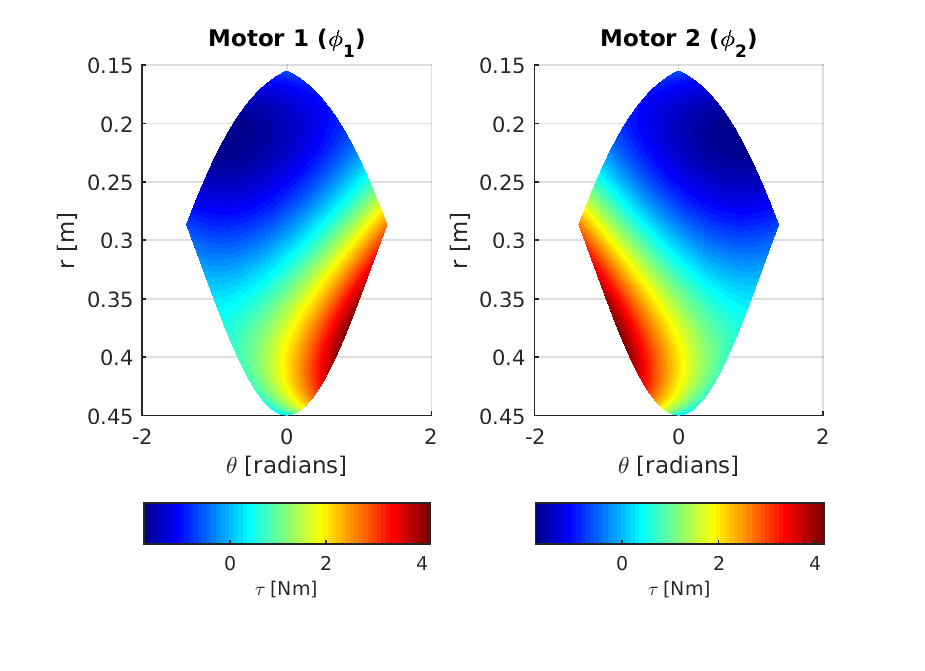
\includegraphics[width=0.8\textwidth]{images/control/forward-kinematic-motor-torque-s-0.eps} 
}

\subfloat[][Caption]{
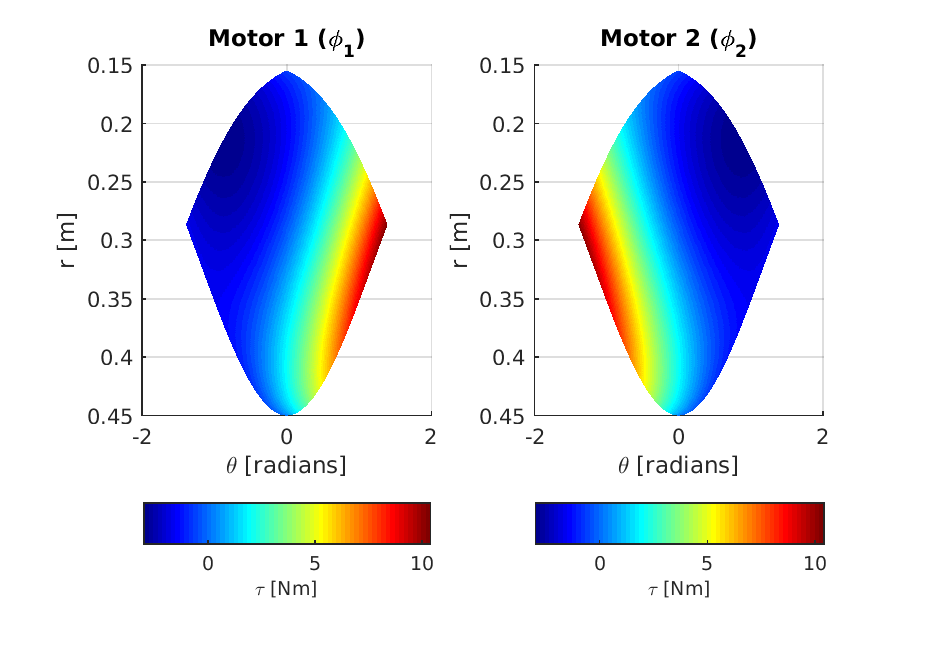
\includegraphics[width=0.8\textwidth]{images/control/forward-kinematic-motor-torque-theta-0.eps} 
}
\caption{Polar co-ordinate spring force mapping to motor torque.}
\label{fig:Polar co-ordinate spring force mapping to motor torque}
\end{figure}

\begin{figure}
\centering
\subfloat[][Caption]{
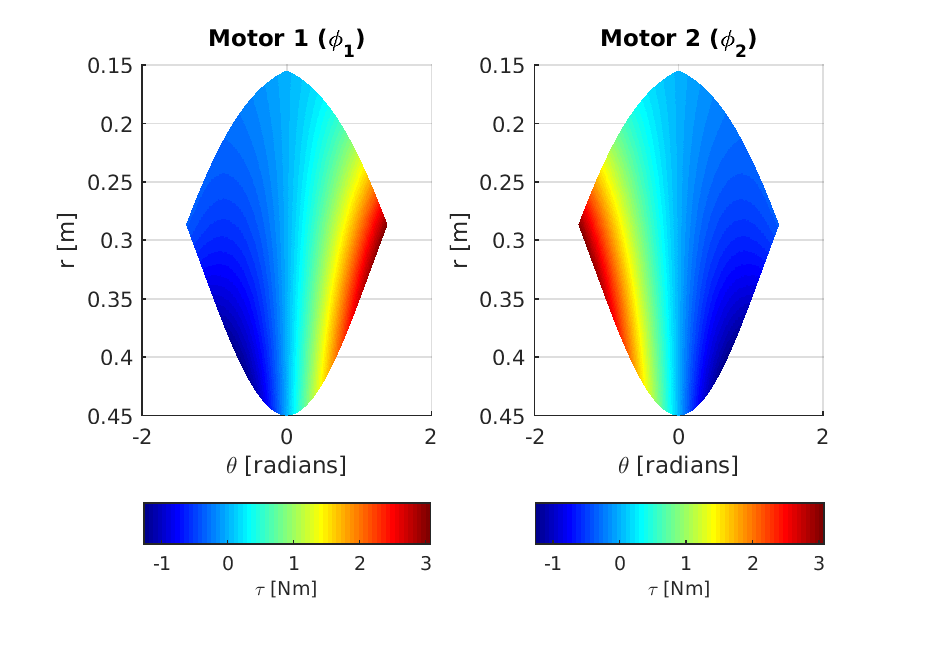
\includegraphics[width=0.8\textwidth]{images/control/forward-kinematic-motor-torque-s-only-0.eps} 
}

\subfloat[][Caption]{
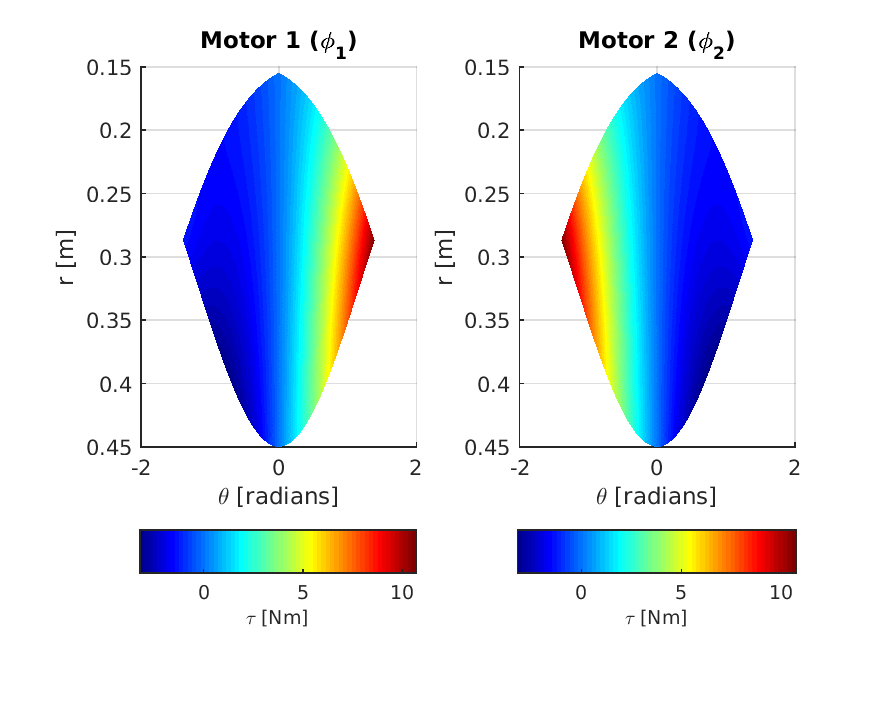
\includegraphics[width=0.8\textwidth]{images/control/forward-kinematic-motor-torque-theta-only-0.eps} 
}
\caption{Polar co-ordinate spring force mapping to motor torque.}
\label{fig:Polar co-ordinate spring force mapping to motor torque}
\end{figure}

\begin{equation}
\tau = J^TF
\end{equation}

\subsection{Current Control}
\label{sec:Current Control}

\begin{figure}
\centering
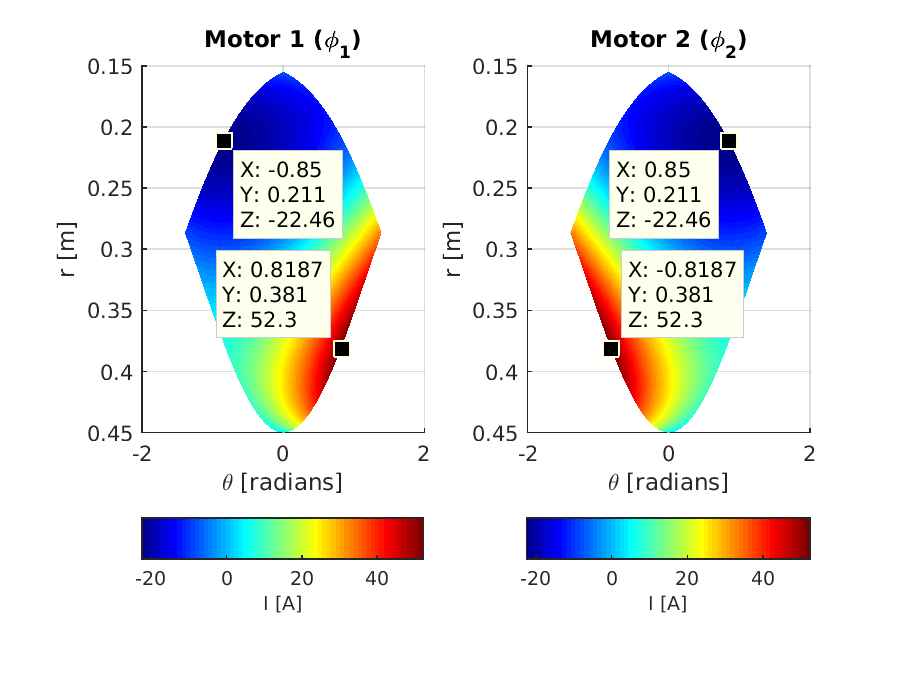
\includegraphics[width=1\textwidth]{images/control/forward-kinematic-motor-current.eps} 
\caption{Active compliance motor current requirements.}
\label{fig:motor-current-requirements}
\end{figure}

\section{Control Loop Design}
\Cref{fig:virtual-model-impedance-loop} is an adaptation of the control loop design found in \cite{Kalouche2016}. Continuous position loop gain scheduling vs virtual spring-damper gain scheduling.

\begin{figure}
\centering
\includegraphics[clip, trim=2cm 8cm 5cm 3cm, page = 1, width=1\textwidth]{images/control/virtual-model-impedance.pdf} 
\caption{Virtual model impedance control loop.}
\label{fig:virtual-model-impedance-loop}
\end{figure}

\subsection{Current Control for Impulse Launch}

Current saturation at 60A.

\section{Torsional Spring-damper}


\subsection{Force Normalisation}

In previous studies using controllers for legs of similar topology, such as those by Duperret et al \cite{Duperret} and Kalouche \cite{Kalouche2016}, Cartesian coordinate systems have been used for virtual model compliance control in the case of \cite{Kalouche2016} and in the case of \cite{Duperret} a Raibert type controller was used with a polar coordinate system.

The study by Kalouche \cite{Kalouche2016} used a convenient coordinate system that had all axis of foot force and placement control in the same unit of measurement, namely distance in meters. 

By using a polar coordinate system virtual model compliance control is made more intuitive as further developed in \cref{chap:Geometry} and \cref{chap:Dynamic Modelling}. 

The drawback to the classic polar coordinate system is the different units of measurement for radial $[m]$ and angular $[radians]$ measure. When applying torsional spring-damper dynamics to the model via control this results in vastly disproportionate force vectors that when mapped to motor torques via the Jacobian, derived in \cref{chap:Kinematics}, result in an unstable control system unless the foot force components are properly scaled. 

An elegant solution to this problem and a way to normalise the angular foot force component is to use the relation in \cref{eq:arc-length-mapping} and visualised in \cref{fig:Arc-length vs. radian measure geometry}.

\begin{equation}
s = r \theta
\end{equation}

\begin{figure}
\centering
\includegraphics[clip, trim=2cm 8cm 2cm 2cm, page=1, width=0.5\textwidth]{images/control/arc-length-theta-geometry.pdf} 
\caption{Arc-length vs. radian measure geometry.}
\label{fig:Arc-length vs. radian measure geometry}
\end{figure}

Using the arc-length of the leg model instead of the radian measure results in a unit of measurement in meters, a more easily interpreted force component, and a better behaviour under ground reaction forces as explained in \cref{sec:Ground Reaction Force}. 

\subsection{Ground Reaction Force}
\label{sec:Ground Reaction Force}

A ground reaction force (GRF) is a force exerted by the ground on a body that is in contact with it. In the case of the leg model it generates a torque around the center of mass of the body. The more distance there is between the center of mass and the ground, the more prominent the ground reaction forces will be. 

There are two ways to deal with ground reaction forces - either by treating them as disturbances in the control model or by making the dynamic model more resilient to the torques generated by GRFs, or perhaps a combination of both. 

The GRFs are most significant during the leg's impact with the ground after flight. During this landing stage all of the kinetic energy of flight is transferred to spring potential energy and damper kinetic energy. The leg radius also changes during this stage which has a direct relationship to torques generated by the GRF around the center of mass. 

By using arc-length for the virtual spring-damper control model it couples the resulting torsional foot force to the GRF torque. The result of this control method, as well as the effect of normalisation of torsional foot forces, is clearly seen in the foot force simulation of \cref{fig:Rotational foot force comparison}. The simulation shows the relation between all possible foot positions in relation to the leg body with a colour map of the resulting torsional foot force at those positions overlayed. This is assuming a spring constant of $30\ Nm$, zero damping, and a rotational set-point of $s = 0\ m$ - visualised in \cref{fig:Leg spring-damper virtual model}.

In \cref{fig:Rotational foot force comparison} as the leg radius, $r\ [m]$, increases the resulting rotational foot force increases. This effect is most pronounced at the maximum rotational off-set where the maximum rotational foot forces are also seen. 

Practically, using arc-length as a measure of rotational off-set for spring-damper virtual model implementation results in a coupling between radial and rotational spring forces. This has beneficial effects on the dynamics and control of the system.

\begin{figure}
\centering
\includegraphics[width=1\textwidth]{images/control/theta-vs-arc.eps} 
\caption{Rotational foot force comparison using angle and arc-length torsional spring virtual model.}
\label{fig:Rotational foot force comparison}
\end{figure}

\section{Full-leg vs. Joint Active Compliance}

The theory of torsional and linear spring-damper systems was developed in \cref{chap:Dynamic Modelling}. Theoretically, if the necessary kinematic and resulting Jacobian mappings can be derived, a torsional or linear spring-damper can be applied in the virtual compliance model around any joint or axis of movement. This leaves endless possibilities for leg virtual compliance topologies.

Two topologies were used in the study \cite{Kalouche2016}, where a slightly different multi DOF leg model was used. Namely full-leg and joint active compliance. For consistency and to compare results with the study, both of these topologies were tested in \cref{chap:Experimental Testing}. 

These two topologies are not intuitively comparable, but by using simulation and performing experimental tests it is possible to compare the two. Realistically the full-leg compliance model is better suited to hopping control because of the polar vs. motor angle orientated general co-ordinates, where foot position can be directly controlled full-leg compliance model.

The full-leg spring-damper model can be visually seen in \cref{fig:Leg spring-damper virtual model} and the joint spring-damper model in \cref{fig:Joint spring-damper virtual model}.

